\section{Improvement-set experiments}\label{sec:set-experiments}
\subsection{Protocol}
This matched-update comparison shares teacher, initial student, pool,
optimizer, refresh and cost gate, without the audit branches. Point
fitting regresses the realized anchor; set fitting recomputes projection
onto $C_\alpha$ at every update; upper-model fitting minimizes
$\mathcal B_z$ normalized by its quadratic coefficient. Point and set
use $\eta=16$. Adaptive point doubles $\eta$ on rejection, invalid
prediction or reduction ratio below 0.25, and halves it above 0.75,
within $[0.25,4096]$.

The teacher is a fixed 30-second checkpoint. Runs use 64 training,
128 validation and 512 disjoint test initials, generated after selected
checkpoint saving; initial cache 512, batch 256, Adam learning rate
0.002 and 1,024 updates. Every 256 updates a training-cost gate rejects
or accepts; rejection restores accepted parameters and Adam always resets.
After update 512, replace half the cache with 256 pairs from accepted
student trajectories on eight training initials. Validation selects
among accepted checkpoints and initialization. Hidden weights and
minibatch seeds are paired within architectures. Sensitivities are exact,
$\varepsilon=0$, with empirical $\kappa=0.000550492$ in mechanics
and $0.000417389$ in reaction.

Exploration uses both tasks, widths 16/64, $\alpha\in\{0.25,0.5,0.75\}$,
and zero residual over the analytic base (24 fits), plus pretrained
width-64 students from the 7.5-second parent (12 fits). Each condition
compares point, adaptive point, upper model and three set relaxations
with one teacher/data seed per task (\ref{app:set-pilots}).
Only pretrained reaction meets the prespecified replication criterion:
at least 1\% validation improvement over both point comparators,
selecting $\alpha=0.25$. Five independent teacher/student/data pairs
then compare this relaxation with the three controls. Pilot samples
are not pooled; paired 95\% $t$ intervals use five seed means without
multiplicity adjustment. Charged time includes graph preparation,
queries, projection, fitting, refresh, gates and validation, excluding
pretraining; wall budgets are not matched.

\subsection{Results}
Exact projection and eight-dimensional quadratic checks are in
\ref{app:set-geometry}.
\begin{figure}[htbp]\centering
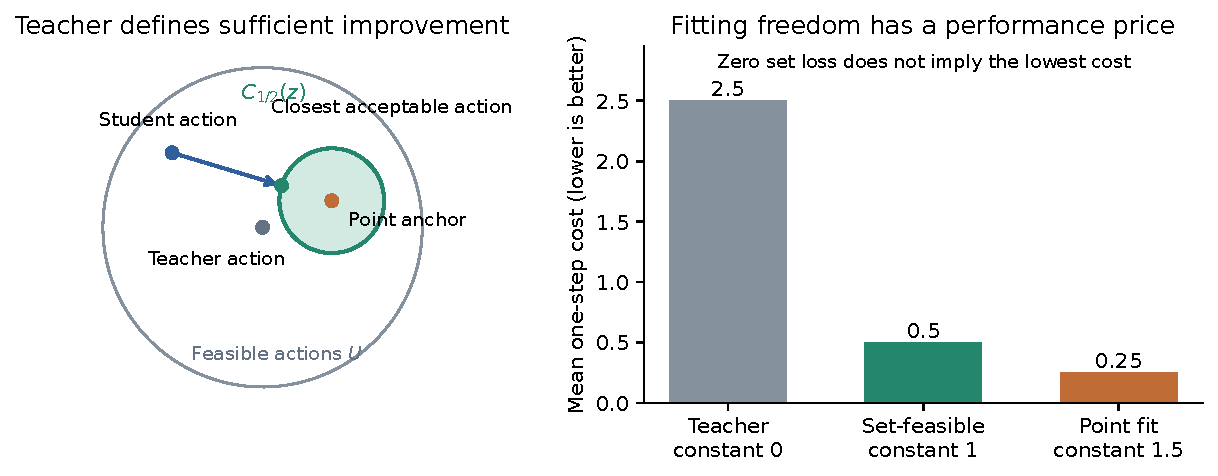
\includegraphics[width=\linewidth]{figures/improving_set_geometry.pdf}
\caption{The teacher supplies an acceptable-improvement set; the student
is pulled toward its closest member. The right panel is the analytic
two-state counterexample, where zero set loss permits a policy with higher
cost than point fitting. These are geometric and analytic illustrations,
not neural-training results.}\label{fig:set-geometry}
\end{figure}
\begin{table}[htbp]\centering\small
\caption{Reaction-task improvement-set replication: five paired seed means after 1,024 updates. Times charge preparation and all teaching operations, with pretraining separate. The selected initial count includes both gate and validation effects.}
\label{tab:set-replication}
\begin{tabular}{lrrr}\toprule
Method & Mean test cost & Charged s & Initial selected \\ \midrule
Point anchor & 0.907593 & 6.524 & 4/5 \\
Adaptive point & 0.907593 & 6.517 & 4/5 \\
Upper model & 0.891263 & 6.523 & 4/5 \\
Set, $\alpha=0.25$ & 0.902697 & 6.570 & 3/5 \\
\midrule
Initial student & 0.908277 & -- & -- \\
Teacher & 0.737725 & -- & -- \\
\bottomrule\end{tabular}\end{table}

Replication gives set cost 0.902697 versus point/adaptive 0.907593
and upper-model 0.891263. Set-minus-point is $-0.004896$
$[-0.041095,0.031303]$, with one win, one loss and three ties;
set-minus-upper is $0.011434$ $[-0.008016,0.030885]$. Set cost
remains 22.36\% above teacher, with no teacher wins.
\begin{figure}[htbp]\centering
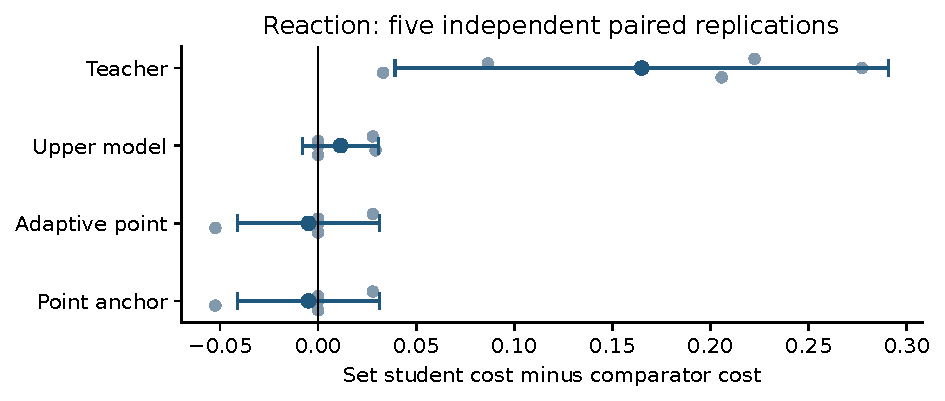
\includegraphics[width=.92\linewidth]{figures/improving_set_replication.pdf}
\caption{Set-student cost minus comparator cost in independent reaction
replications. Small points are the five paired differences; large points
and bars give their means and unadjusted 95\% $t$ intervals. Negative
values favor the set student.}\label{fig:set-replication}
\end{figure}
Initialization is selected in 3/5 set runs and 4/5 comparator runs.
The pretrained pilot lowers validation cost from 1.049305 to 0.938238
but raises test cost from 0.854282 to 0.993972. Analytic-base conditions
give no selected set-policy improvement. All adverse outcomes are retained.

Post-fit probes use 64 pairs per student on four separate trajectories,
with fresh $\eta=16$ anchors and $\alpha=0.25$. On set-student states,
set MSE is $1.36737\times10^{-4}$ versus point MSE
$9.54646\times10^{-4}$; point-trained students have set MSE
$1.28877\times10^{-4}$ on their own states. Membership is 37.5\%
versus 17.19\%, but mean local advantages are $1.4860\times10^{-6}$
versus $-4.8371\times10^{-6}$. Each objective has one upper-model
violation and one non-improving modeled-set member among 320 dependent
sampled pairs. Thus the empirical sets are not certified.
Charged time averages 6.570 seconds for set and 6.524 for point fitting;
the fitting portions are 0.427 and 0.376 seconds.
